\section{Paired Closed-Loop Assessment Protocol}
\label{sec:protocol}
\subsection{Substrate and Randomness}
The FlyWire v783 graph (Fig.~\ref{fig:v9-protocol}) has 138,639 neurons and 15,091,983 signed connection-table rows, each representing multiple contacts. We use the Shiu LIF parameterization\cite{shiu2024drosophila} in Brian~2\cite{stimberg2019brian2}, NumPy backend, 0.1\,ms steps. The original publication used v630. Sensory cells retain 2.2\,ms refractoriness, a stated stimulation variant. Initial states and unmodified weights are restored before each episode; equations and parameters accompany the source.

An assumed receptive-field map supplies geometry-dependent rates up to 150\,Hz to 104 LC4 and 210 LPLC2 cells. Other external rates are zero. Eight descending cells form a synthetic command interface. Anatomy and looming selectivity\cite{klapoetke2017looming} motivate the substrate; the map and body coupling are not validated fly behavior. Actual cell identities and map parameters are saved.

Each seed crosses both bearings, both laws and healthy/25\%/50\% deletion. Shared row variates define $w_j^{(f)}=w_j I(V_{sj}\geq f)$, giving nested masks. All contacts in a row are removed together. Separate frame-indexed uniforms generate inputs $I[U_{sk\tau i}<\lambda_{ki}\Delta t]$. Uniforms are common across conditions; realized events differ through feedback-dependent $\lambda$. Digests bind masks, uniforms, actual events, maps, sources and external tables. Seed traceability does not imply cross-platform bit identity.

\begin{figure*}[t]
\centering
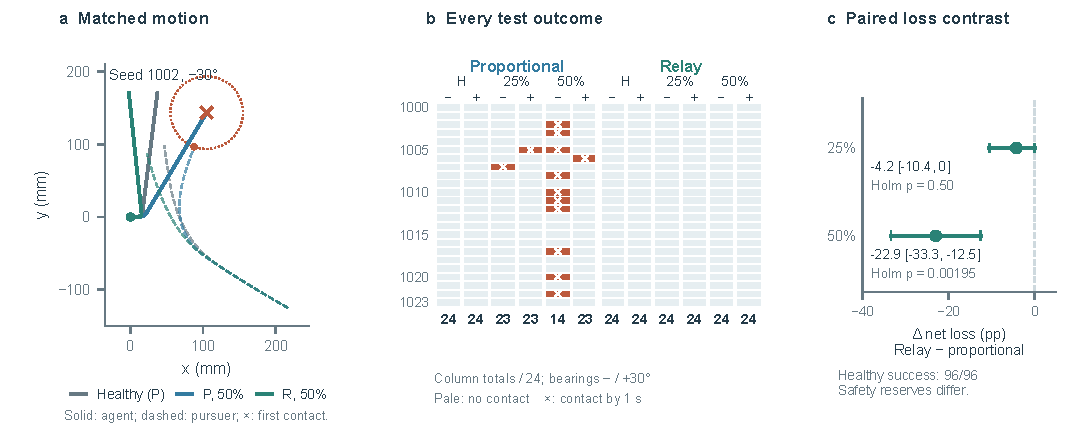
\includegraphics[width=\textwidth]{figs/task_v9_outcomes.pdf}
\caption{Feedback and task loss. (a) Actual matched paths for seed 1002, $-30^\circ$, the first seed-ordered proportional 50\%-deletion collision, shown descriptively. Solid/dashed: agent/pursuer; paths stop at first contact, with 50-mm dotted contact radius. (b) All 288 outcomes in 24 seed rows; column totals are successes/24. Bearings, laws and doses within each seed are paired. (c) Registered relay-minus-proportional net-loss contrasts, 95\% whole-seed bootstrap intervals and Holm-adjusted $p$. Healthy safety reserves differ.}
\label{fig:v9-outcomes}
\end{figure*}

\subsection{Causal Feedback and Actuation}
Body-frame bearing subtracts heading from world-relative bearing. Looming uses changes in $\alpha=\arctan(0.05/d)$ at actual separation $d$. Input begins at 100\,ms; decisions at each frame end affect the \emph{next} 20\,ms motion interval.

Twenty passive episodes (four seeds; $-60,-30,0,30,60^\circ$) fit a ridge decoder $z_k=\beta_0+\boldsymbol\beta^\top\bar{\mathbf r}_k$ of bearing/$60^\circ$, using five-frame means of eight command rates. Both laws set $\omega_k=0$ before the cue or below the 4.03125\,Hz eight-cell mean trigger level; otherwise
\begin{equation}
\omega_k=\begin{cases}
-600\operatorname{clip}(z_k,-1,1),&\text{proportional},\\
-600\operatorname{sgn}(z_k),&\text{relay},
\end{cases}\quad[\mathrm{deg/s}].
\end{equation}
The first qualifying decision $t_d$ schedules one 0.35\,m/s heading-fixed burst on $[t_d+250,t_d+700)$\,ms. Otherwise speed is 0.05\,m/s and heading is capped at $\pm100^\circ$. Motion segments split at exact actuator boundaries; positions use starting heading, updated at each segment end. A 0.3\,m/s pursuer starts 0.25\,m away and aims at the agent at each segment's beginning. First contact at distance $\leq0.05$\,m is solved inside each linear relative-motion segment.

Success means collision-free through 1\,s, not eventual escape. Walk-only segments satisfy $d_{\rm next}\leq d-0.25\delta$ ($\delta$ in seconds), so contact occurs by 0.8\,s without a burst in this plant. Failure latches at first contact; the trajectory and neural loop continue for equal 1\,s resource exposure. Post-contact activity is counterfactual accounting, not physical collision dynamics or warning data. Independent replay checks inputs, geometry, decisions, clocks and horizon state without rerunning neural dynamics.

\subsection{Paired Estimands}
Let $S_F(t),S_H(t)$ be paired network counts, and $T_F,T_H$ their contact-frame end or 1\,s. With $T_*=\min(T_F,T_H)$, distinguish
\begin{equation}
R_{\rm stop}=\frac{S_F(T_F)}{S_H(T_H)},\quad
R_{\rm common}=\frac{S_F(T_*)}{S_H(T_*)}.
\end{equation}
Fixed 400\,ms and 1\,s ratios are separate estimands. The former precedes all contacts; common duration remains outcome-dependent and does not equate sensory histories. For binary outcomes, report loss $Y_H(1-Y_F)$, gain $(1-Y_H)Y_F$ and net loss $D=Y_H-Y_F$. The controller interaction is $D_{\rm relay}-D_{\rm proportional}$, averaging bearings within seed.

\subsection{Validation, Warnings and Inference}
An initial controller failed its declared capability screen; all attempts are retained. Final calibration passed on eight new healthy validation clusters, 8/8 per law/bearing. A two-cluster fault screen was developmental. Core testing uses 24 new clusters (288 episodes); eight separate $\pm45^\circ$ clusters test angle transfer. Parameters, thresholds and stopping rules were frozen before both tests.

Warnings use only data through 400\,ms: low mean command rate, an upper activity limit, and $|\log(S/\tilde S_H)|$ against law/side-specific healthy medians. A held-command forecast uses current geometry, neural turn command and pending burst; absent a trigger it assumes the earliest next-frame decision. A same-state actuator baseline sets future turn to zero. Both have exact simulated geometry, not implemented sensors or reachability guarantees. Lower fifth-percentile command/clearance and upper 95th-percentile log-score thresholds use all healthy validation records. Cutoffs are 5.833\,Hz (100--400\,ms command mean), activity ratios outside $[0.844,1.185]$, and predicted clearance below 18.77/18.55\,mm for held-command/schedule forecasts. The upper resource limit is $2\tilde S_H$. Healthy flag calibration does not guarantee task false-alarm rates.

All test records contribute sensitivity, specificity, false alarms and misses against contact through 1\,s. Confidence intervals use 20,000 whole-seed percentile resamples, RNG 20261022. Controller sign-flip sensitivity assumes a symmetric cluster null, Holm-adjusted over two doses. Fixed 800/900/1000\,ms task horizons are repeated observations, not new replicates. No test tuning, seed replacement or efficacy stopping is permitted. Inference remains conditional on one model, map and task.
